\documentclass[varwidth=true, border=2pt]{standalone}
\usepackage{tikz}
\usetikzlibrary{patterns,calc,decorations.markings}

\begin{document}
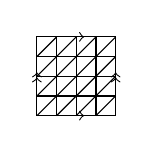
\begin{tikzpicture}
    \node (a) at (0,0) {};
    \node (b) at (1,0) {};
    \node (c) at (1,1) {};
    \node (d) at (0,1) {};
    \coordinate (m) at ($(a)!0.5!(c)$);
    \coordinate (ab2) at ($(a)!0.5!(b)$);
    \coordinate (ab1) at ($(a)!0.5!(ab2)$);
    \coordinate (ab3) at ($(b)!0.5!(ab2)$);
    \coordinate (bc2) at ($(b)!0.5!(c)$);
    \coordinate (bc1) at ($(b)!0.5!(bc2)$);
    \coordinate (bc3) at ($(c)!0.5!(bc2)$);
    \coordinate (cd2) at ($(c)!0.5!(d)$);
    \coordinate (cd1) at ($(c)!0.5!(cd2)$);
    \coordinate (cd3) at ($(d)!0.5!(cd2)$);
    \coordinate (ad2) at ($(a)!0.5!(d)$);
    \coordinate (ad1) at ($(a)!0.5!(ad2)$);
    \coordinate (ad3) at ($(d)!0.5!(ad2)$);
    \draw (a.center) -- (b.center) -- (c.center) -- (d.center) -- cycle;
    %horizontal
    \draw (bc1.center) -- (ad1.center);
    \draw (bc2.center) -- (ad2.center);
    \draw (bc3.center) -- (ad3.center);
    %vertical
    \draw (ab1.center) -- (cd3.center);
    \draw (ab2.center) -- (cd2.center);
    \draw (ab3.center) -- (cd1.center);
    %diagonal
    \draw (ad3.center) -- (cd3.center);
    \draw (ad2.center) -- (cd2.center);
    \draw (ad1.center) -- (cd1.center);
    \draw (a.center)   -- (c.center);
    \draw (ab1.center) -- (bc3.center);
    \draw (ab2.center) -- (bc2.center);
    \draw (ab3.center) -- (bc1.center);
    \begin{scope}[decoration={
        markings,
        mark=at position 0.6 with {\arrow{>}}}
    ] 
        \draw[postaction={decorate}] (a.center) -- (b.center);
        \draw[postaction={decorate}] (d.center) -- (c.center);
    \end{scope}

    \begin{scope}[decoration={
        markings,
        mark=at position 0.55 with {\arrow{>>}}}
    ] 
        \draw[postaction={decorate}] (b.center) -- (c.center);
        \draw[postaction={decorate}] (a.center) -- (d.center);
    \end{scope}
\end{tikzpicture}
\end{document}
